\documentclass{beamer}
\usepackage{graphicx}
\usetheme{Madrid}

% Title page information
\title{COMP 354 Iteration 1 Eternity Project}

\subtitle {Team I}

\author
{
Hong Phuc Nguyen \\ Swati Pareek \\Anik Patel\\Avnish Patel 
\\Clément Potteck \\ Tara Seal \\Emanuel Sharma
}

\institute{
Concordia University
}
\date{Friday June 5, 2020}

\begin{document}

\frame{\titlepage}

% wondering if the TOC is necessary for a 10-min presentation?
% I would agree about title pages separating main sections though
\begin{frame}
\frametitle{Overview}
\tableofcontents
\end{frame}

\section{Team}



\begin{frame}
\frametitle{The Team}
\null\hfil\hfil\makebox[2cm]{Nguyen}
\hfil\hfil\makebox[2cm]{Swati}
\hfil\hfil\makebox[2cm]{Anik}
\hfil\hfil\makebox[2cm]{Avnish}
\newline
\hfil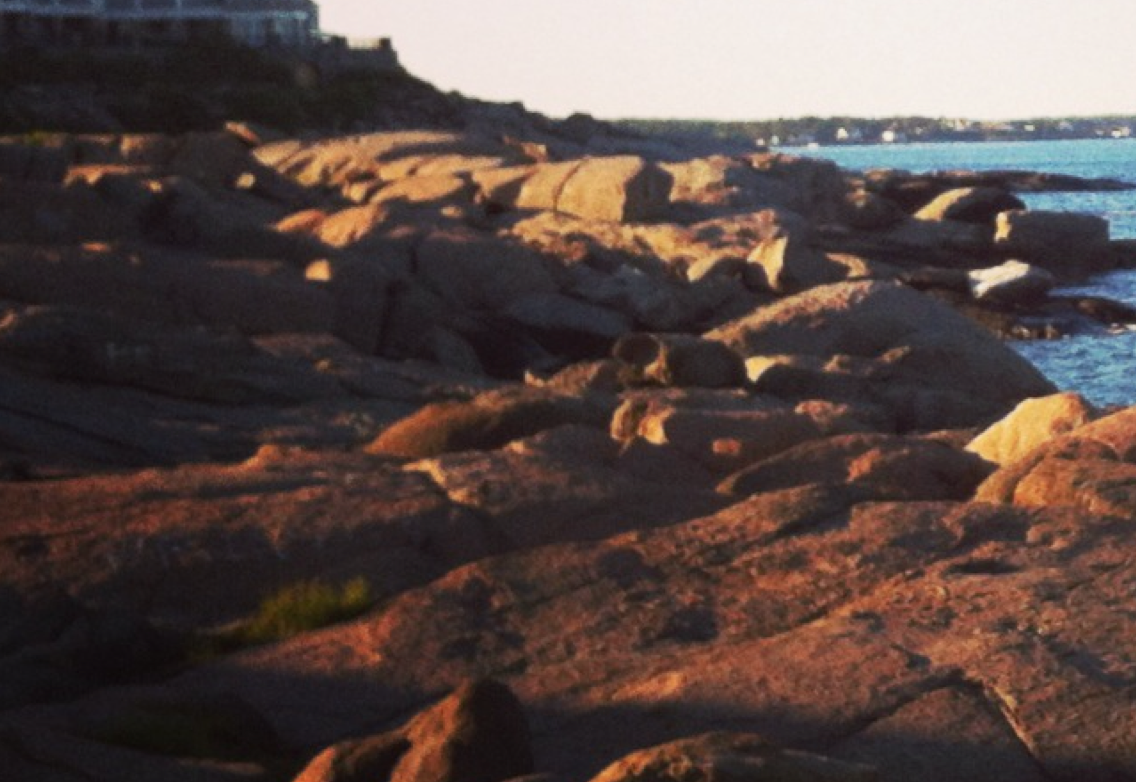
\includegraphics[width=2cm]{Screen Shot}
\hfil\hfil\hfil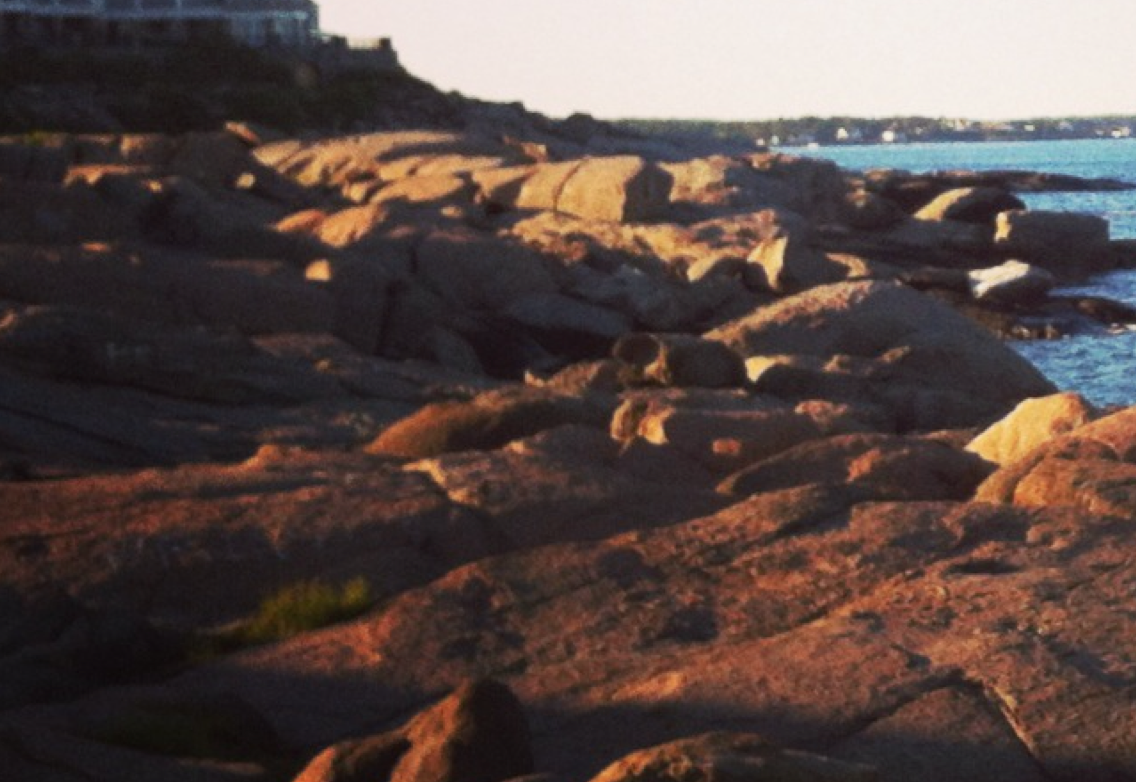
\includegraphics[width=2cm]{Screen Shot}
\hfil\hfil\hfil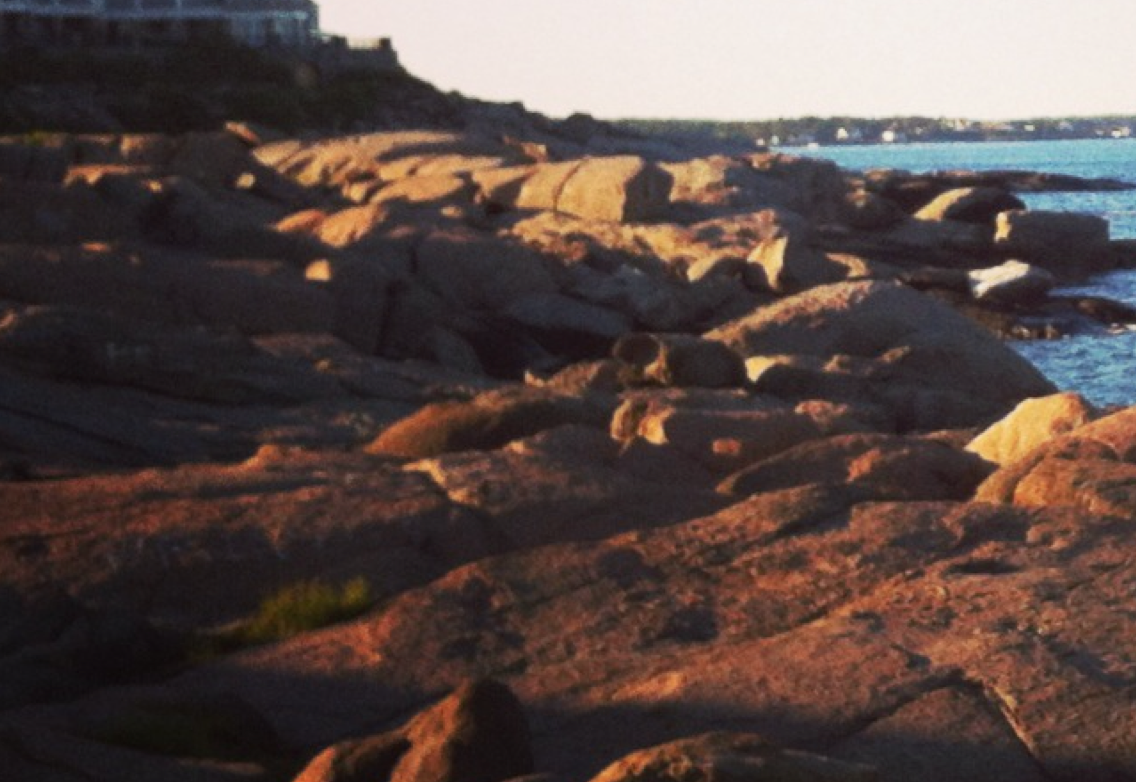
\includegraphics[width=2cm]{Screen Shot}
\hfil\hfil\hfil\hfil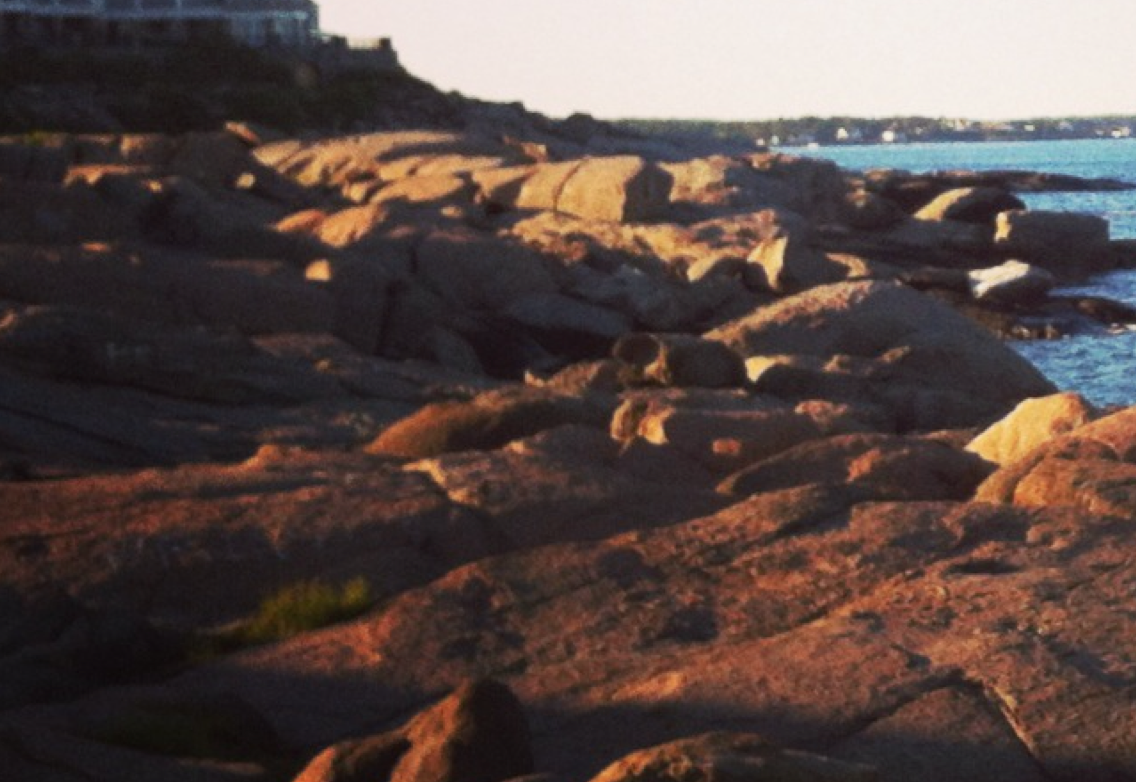
\includegraphics[width=2cm]{Screen Shot}\newline
\null\hfil\hfil\makebox[2cm]{MAD}
\hfil\hfil\makebox[2cm]{\[e^x\] XOR \[a^x\]}
\hfil\hfil\makebox[2cm]{sin(x) XOR cos(x)}
\hfil\hfil\makebox[2cm]{sinh(x)}
\newline\newline
\vfil
\null\hfil\hfil\makebox[2cm]{Clément}
\hfil\hfil\makebox[2cm]{Tara}
\hfil\hfil\makebox[2cm]{Emanuel}\newline
\hfil\hfil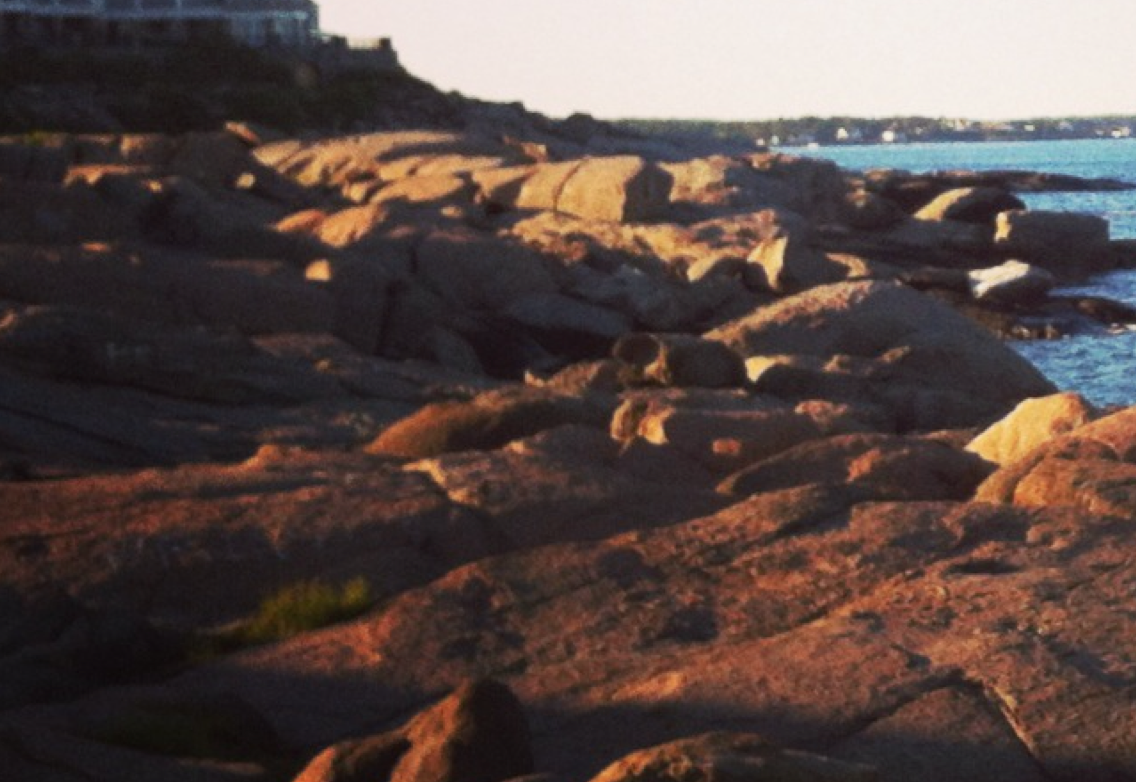
\includegraphics[width=2cm]{Screen Shot}
\hfil\hfil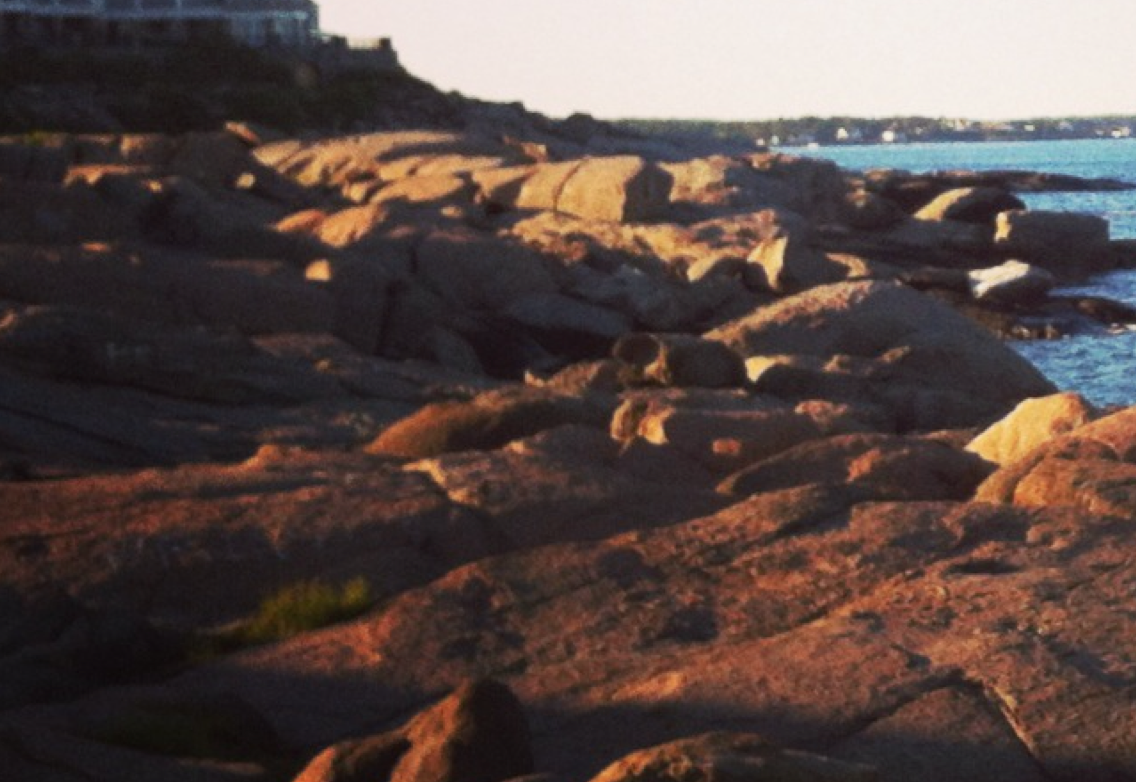
\includegraphics[width=2cm]{Screen Shot}
\hfil\hfil\hfil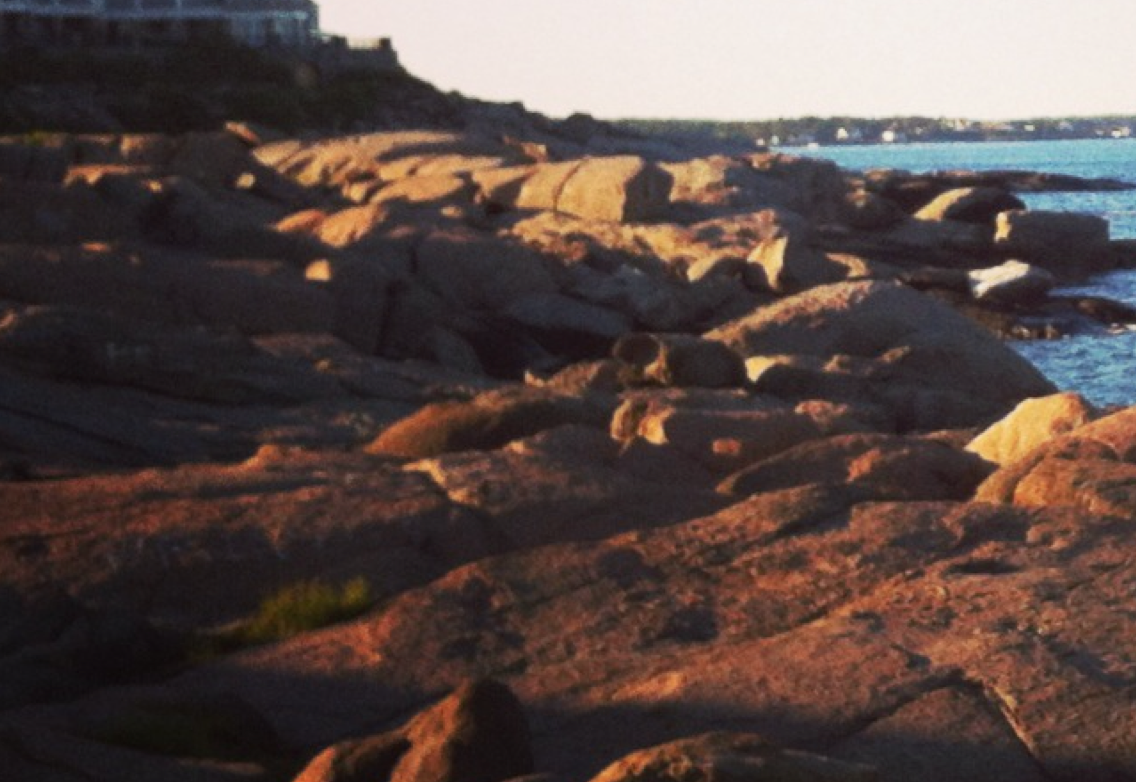
\includegraphics[width=2cm]{Screen Shot}\newline
%There's an error about the dollar sign with these functions
\null\hfil\hfil\makebox[2cm]{\[10^x\] XOR \[\Pi^x\]}
\hfil\hfil\makebox[2cm]{\[x^y\]}
\hfil\hfil\makebox[2cm]{ln(x) XOR log_1_0(x) }\newline
\end{frame}



  \begin{frame}
\frametitle{Team Roles}
\small
\begin{table}
\begin{tabular}{l | c | c | c | c }
Name & Primary Role and Responsibility & Secondary Role \\
\hline
Hong Phuc & GUI and Web application,& Implementation of\\
& prototyping & new technologies\\
\hline
Swati & Organizing and planning agenda& High-level vision, \\
& for team meetings & scope management\\
\hline
Anik & Set up of initial repository& Questions regarding\\
& GUI for local application & the Python ecosystem\\
\hline
Avnish & Technical Writer & Latex \\
\hline
Clément & Major presenter, & Best practices, \\
& quality control  & PEP documentation\\
\hline
Tara & Minor presenter, & Ensuring requirements \\
& Team liason  & are followed\\
\hline
Emmanuel & Technical writer, &  Algorithm optimization\\
& subject matter expert  & \\
& for math algorithms  & \\
\end{tabular}
\end{table}
\end{frame}

\begin{frame}
\frametitle{Collaboration patterns:\\ Managing the project}
\begin{itemize}
 \item Regular meetings once a week
 \item Agenda
   \begin{itemize}
   \item Keeps meetings focused and on track
   \item Meeting transcriber ensures that discussions are on track with agenda
   \end{itemize}
 \item Questions and Answers
    \begin{itemize}
   \item Questions are gathered by the meeting transcriber
   \item Questions are sent to the professor
   \end{itemize}
 \item Status Update: done, doing, to-do
 \item Follow up on decisions and commitments
\end{itemize}
\end{frame}

\begin{frame}
\frametitle{Collaboration Patterns: \\ Centralizing work product management}
\begin{itemize}
 \item Focus on real-time information and feedback
 \item Discord
  \begin{itemize}
   \item Group channels: chat, pings, pins
   \item Direct Messages: on-on-one conversations
   \item integrated voice calls for meetings
  \end{itemize}
 \item Google Drive
 \item GitHub
  \begin{itemize}
   \item Quality Control: protected branches
     \begin{itemize}
        \item protected branches
        \item staging branch
        \item master branch
    \end{itemize}
   \item Required asymmetric code reviews
  \end{itemize}
\end{itemize}
\end{frame}


%Slide for future directions
\begin{frame}
\frametitle{Code Reviews}
 \begin{itemize}
  \item One individually assigned to each Pull Request
  \item Asymmetric
  \item Additional techniques used:
   \begin{itemize}
    \item Inputs and discussion from all team members encouraged
    \item Continuously enforce quality standards
   \end{itemize}
\end{itemize}
\end{frame}



\section{Requirement Gathering}

% Slide for the interview questions
\begin{frame}
\frametitle{Interview Questions}
\begin{itemize}
 \item Demographic of people who use a calculator
  \begin{itemize}
   \item Professional/educational background
   \item Calculator Usage
  \end{itemize}
 \item User needs
  \begin{itemize}
   \item Degree of precision
   \item Input box vs. button selection
   \item Numeral system required
  \end{itemize}
 \item Separate requirements into needs and preferences
  \begin{itemize}
   \item Ease of use
   \item Aesthetics
   \item Features
   \item Platform
  \end{itemize}
   \item Frustrations with current device
\end{itemize}
\end{frame}


%Slide for the interview model
\begin{frame}
\frametitle{Interview Model}
\begin{itemize}
 \item Hourglass
  \begin{itemize}
   \item General questions asking the user to describe what they do and how they use a calculator
   \item Specific questions related to their work
   \item Ended interview with an open-ended question to see if there is anything they'd like to add
  \end{itemize}
 \item Findings
  \begin{itemize}
   \item Many interviewees went back to previous questions we asked during the open-ended question at the end to clarify something they said.
  \end{itemize}
\end{itemize}
\end{frame}


  %Slide for our interview findings
\begin{frame}
\frametitle{Interview: Key findings}
\begin{itemize}
 \item Precision is extremely important
 \item Existing calculators contain a lot of unnecessary buttons and features
 \item Split findings on local or web application
  \begin{itemize}
   \item Mobility when conducting experiments or for exams
   \item Preference for desktop application when working at computer
  \end{itemize}
\end{itemize}
\end{frame}




%Slide for our use case
\begin{frame}
\frametitle{Summarized Use case}
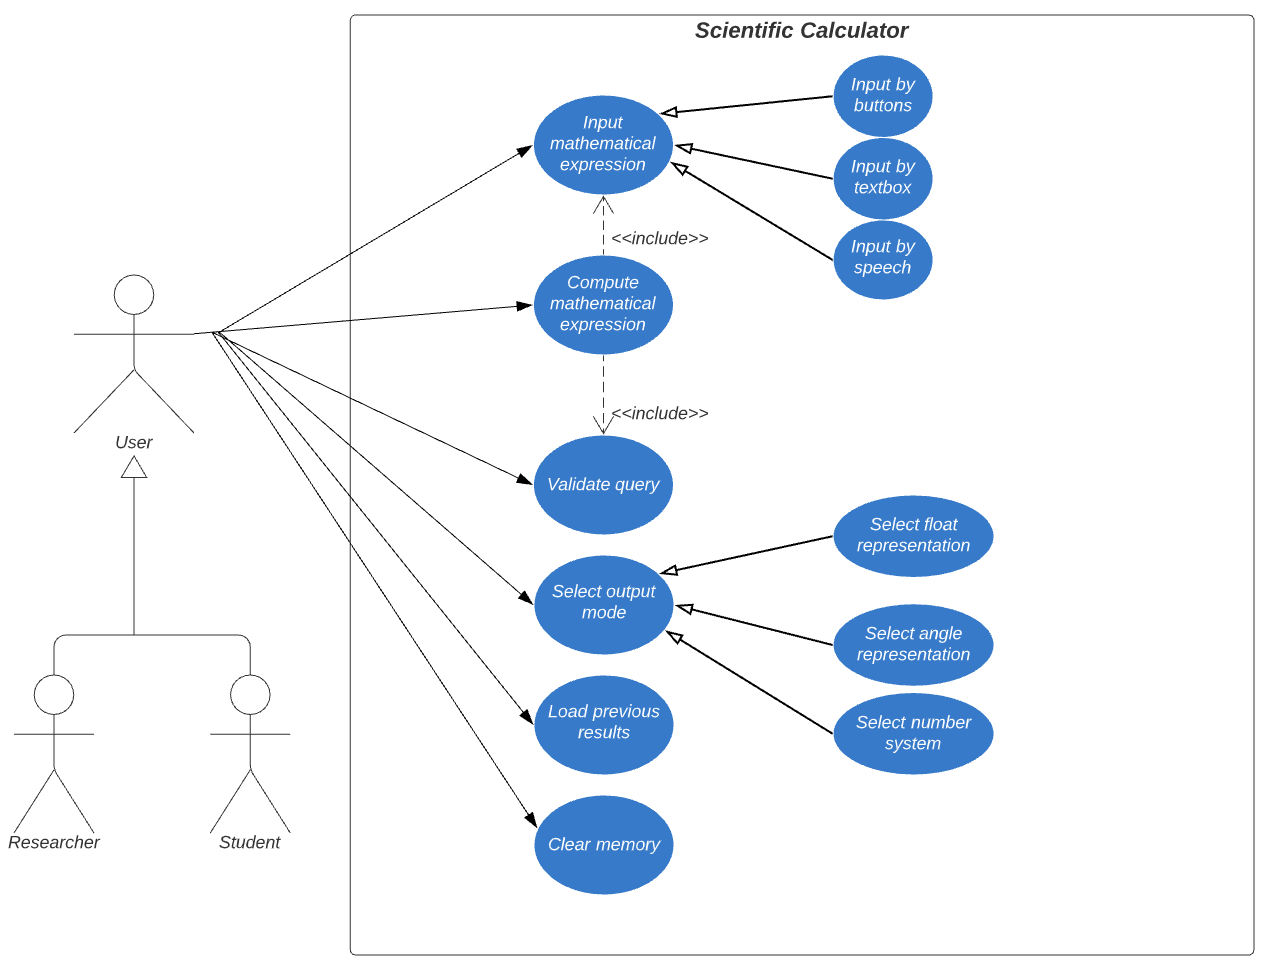
\includegraphics[scale=0.5]{Use Case}
\end{frame}



\begin{frame}
\frametitle{Tech Stack}
 \begin{itemize}
  \item choice of technologies influenced by team strengths and user requirements
  \item python: familiar \& versatile
   \begin{itemize}
    \item a language we were all comfortable with
    \item rapid iterations
    \item option of a GUI vs. CLI calculator
    \item native language recognition libraries
   \end{itemize}
  \item keeping our options open:
   \begin{itemize}
    \item electron for a local desktop front-end
    \item flask or nodejs for a web implementation
   \end{itemize}
  \end{itemize}
\end{frame}

\begin{frame}
\frametitle{Inclusions/Exclusions}
\begin{itemize}
 \item Information from users gave us a clear idea on what should be built
  \begin{itemize}
  \item Some ideas were not feasible in the timeframe
  \begin{itemize}
    \item Speech recognition
    \item Radian and degree conversions
  \end{itemize}
  \item Scope \& reasoning
    \begin{itemize}
    \item Essential features/functionality - for iteration 1
    \item Features/functionality to be looked at a later point
  \end{itemize}
  \end{itemize}
  \end{itemize}
\end{frame}

%Slide for future directions
\begin{frame}
\frametitle{Iteration 2: Organizational improvements}
\begin{itemize}
 \item Collaboration techniques
  \begin{itemize}
   \item Buddy system
   \item Role rotation
   \item Better project \& team wiki
  \end{itemize}
\end{itemize}
\end{frame}

%Slide for future directions
\begin{frame}
\frametitle{Product}
\end{frame}

\section{Product}
\begin{frame}
\frametitle{References}
\end{frame}

\end{document}
